\documentclass[conference,onecolumn, catalan]{IEEEtran}
\IEEEoverridecommandlockouts
% The preceding line is only needed to identify funding in the first footnote. If that is unneeded, please comment it out.
\usepackage{comment}
\usepackage{hyperref}
\usepackage{cite}
\usepackage{amsmath,amssymb,amsfonts}
\usepackage{algorithmic}
\usepackage{textcomp}
\usepackage{xcolor}
\def\BibTeX{{\rm B\kern-.05em{\sc i\kern-.025em b}\kern-.08em
    T\kern-.1667em\lower.7ex\hbox{E}\kern-.125emX}}
\newtheorem{theorem}{Teorema}
\usepackage{listings}
\usepackage{babel}
\usepackage{geometry}% http://ctan.org/pkg/geometry
\usepackage{graphicx}% http://ctan.org/pkg/graphicx
\usepackage{color} %red, green, blue, yellow, cyan, magenta, black, white
\definecolor{mygreen}{RGB}{28,172,0} % color values Red, Green, Blue
\definecolor{mylilas}{RGB}{170,55,241}
\lstset{language=Matlab,%
    %basicstyle=\color{red},
    breaklines=true,%
    morekeywords={matlab2tikz},
    keywordstyle=\color{blue},%
    morekeywords=[2]{1}, keywordstyle=[2]{\color{black}},
    identifierstyle=\color{black},%
    stringstyle=\color{mylilas},
    commentstyle=\color{mygreen},%
    showstringspaces=false,%without this there will be a symbol in the places where there is a space
    numbers=left,%
    basicstyle=\small,
    numbers = none,
    %numberstyle=none,% size of the numbers
    %numbersep=2pt, % this defines how far the numbers are from the text
    emph=[1]{for,end,break},emphstyle=[1]\color{red}, %some words to emphasise
    %emph=[2]{word1,word2}, emphstyle=[2]{style},    
}

\newenvironment{changemargin}[2]{%
\begin{list}{}{%
\setlength{\topsep}{0pt}%
\setlength{\leftmargin}{#1}%
\setlength{\rightmargin}{#2}%
\setlength{\listparindent}{\parindent}%
\setlength{\itemindent}{\parindent}%
\setlength{\parsep}{\parskip}%
}%
\item[]}{\end{list}}

\title{Segon Informe de Progrés del TFG: \\ \vspace{0.2cm} {\huge \textit{ Desenvolupament d'un ``core" didàctic de RISC-V\ }} }
\author{
\IEEEauthorblockN{Pau Casacuberta Orta}
\IEEEauthorblockA{
\textit{Autonomous University of Barcelona}\\
Cerdanyola del Vallès, Barcelona 08193\\
pau.casacubertao@e-campus.uab.cat\\}}

\usepackage[owncaptions, tablegrid]{vhistory}
\renewcommand{\vhhistoryname}{Històric de versions}
\renewcommand{\vhversionname}{Versió}
\renewcommand{\vhdatename}{Data}
\renewcommand{\vhauthorname}{Autor(s)}
\renewcommand{\vhchangename}{Descripció}
\newcommand\todo[1]{\textcolor{red}{#1}}

\usepackage{pdfpages}

\usepackage{setspace}

% Per a revisió Afegir doble espaciat
\doublespacing


\begin{document}


\maketitle

\textbf{\textit{**Aquesta versió del document és a doble espaiat per a poder facilitar l'anotació de correccion**}}
\begin{versionhistory}
    \vhEntry{0.1}{9.12.19}{Pau}{Creació del primer esborrany.}
    \vhEntry{1.0}{14.12.19}{Pau}{Primera versió del document amb proposta de l'índex de la memòria}
\end{versionhistory}


\begin{abstract}
La finalitat d'aquest document és el de consignar els avenços efectuats en el desenvolupament del treball. També s'inclou una versió preliminar del index del informe final.
\end{abstract}



\section{Seguiment}

En aquesta etapa principalment s'ha sintetitzat del codi verilog del nucli per a implementar-ho en una FPGA i s'està adaptant el nucli per a que pugui funcionar en una plataforma (com la de pulpino), i així poder utilitzar perifèrics directament.


\subsection{FPGA}

Per a poder demostrar que el disseny que s'està desenvolupant en aquest TFG es va proposar fer una implementació en una FPGA, concretament en la plataforma DE0 d'Altera \cite{technologies_terasic_nodate}. Els passos que s'han seguit per a obtenir un model funcional del nucli sobre aquesta plataforma han sigut els següents:

\todo{Afegir descripció del top que realment està a la FPGA, debounce per als botons, clock controlat per botons, 7seg disp per indicar PC.}

\subsubsection{Instal·lació de l'entorn de desenvolupament (Quartus II)}

L'eina principal que s'ha utilitzat per dur a terme la programació de la FPGA és Quartus II web edition 13.0 \cite{jose_quartus_2013} d'Intel, anteriorment Altera. Aquest software està disponible de forma oberta a la pàgina de suport d'Intel. Addicionalment a aquest software ha sigut necessari descarregar els documents que descriuen la FPGA en si per a poder generar l'estructura interna de portes lògiques, disponible a la mateixa pàgina del software.

\subsubsection{Sintetitzar el codi original }

Un cop es tenen les eines instal·lades s'han agafat els fitxers verilog que descriuen el nucli i s'han importat en un projecte especificant la plataforma on es programarà finalment, en aquest cas la FPGA Cyclone III 3C16. 

Per recomanació d'en Raimon s'intenta compilar cada fitxer per separat per a poder arreglar alguns error de compilació abans de fer la sinterització. Un cop el codi compila completament es fa una síntesi del disseny. Aquest disseny mostra que hi ha algun ``Latchs'' que s'han generat de manera automàtica degut hi ha parts que s'esperen que siguin combinacionals però no s'han determinat correctament tots els casos possibles això provoca que per defecte el senyal afectat mantingui el valor, per això la creació del element de memòria. 

\subsubsection{Eliminar els Latchs }

Per a mitigar l'aparició d'elements de memòria no esperats en circuits dissenyats coma combinacionals fa falta identificar quines senyals es veuen afectades per aquest comportament, això es pot veure de manera directa amb l'eina de navegació del disseny RTL. Un cop detectades aquestes senyals modificant el codi original fent que aquestes senyals sempre quedin definides per a un valor, per exemple posant aquest a ``0''. 

\todo{Afegir figura mostrant exemple de codi abans i després (github commit ****)}


\subsection{Megawizard mems}

Degut a que el disseny del \verb|top.v| incorpora les memòries de programa i dades aquestes també es sintetitza discretament amb elements de memòria que al final s'acaben implementant amb portes lògiques. Per a millorar el rendiment, reduir l'àrea de la FPGA i reduir el temps de síntesi s'ha proposat a la reunió utilitzar una eina que proporciona el software (Mega Wizard) per a generar les memòries utilitzant uns mòduls específics que disposa la FPGA per a implementar memòries. Això proporciona un disseny més compacte a la FPGA i amb un rendiment més realista.

\subsubsection{Instancia de les Memòries}

A l'hora d'utilitzar aquestes memòries han sorgit diferents problemes, no en l'etapa de definició dels elements i assignació de recursos a la FPGA, però sí a l'hora d'inicialitzar els valors d'aquestes. En el cas de la memòria de dades no és rellevant però en el cas de la memòria de programa si que suposa un problema. Al final s'ha decidit una manera manual (però fàcilment automatitzable amb scripts externs a les eines proposades) per a generar el document d'inicialització de les memòries a partir del codi compilat per el riscv-gnu-toolkit proporcionat per la risc-v fundation.

\subsubsection{Compilació del programa} complicada, llibreries de sistema

Per obtenir les paraules de memòria que s'hauran de carregar a la memòria de programa que representaran el programa a executar es segueixen els següents passos: primer generar un codi en C per a poder executar-lo en la FPGA, després és necessari utilitzar les eines de compilació proporcionades per el riscv-gnu-toolkit (en concret el compilador gcc) i finalment fer un bolcat del binari generat a la memòria de programa generada a la FPGA. 

Per defecte el compilador gcc afegeix llibreries de sistema operatiu per a control del sistema, degut a que en el nostre cas es una solució encastada i no requereix sistema operatiu s'ha decidit descartar aquestes llibreries per a que en el binari resultant només s'hi acabi compilant el programa escrit en C.

\subsection{RAM-MUX}

Per adaptar el nucli a altres plataformes ja creades la part principal per a que pugui funcionar correctament és fer compatible la manera en la que s'accedeix a les memòries i per exemple poder limitar-ne L'accés si aquest recurs no està disponible. Aquest és el cas de la plataforma pulpino, que utilitza uns elements entre les memòries i el nucli que permeten connectar un bus entremig per afegir perifèrics. Per adaptar el nucli s'ha decidit fer un entorn semblant al de pulpino aprofitant els element que estan entre les memòries i el nucli per a que el nucli generi les senyals necessàries per a funcionar com s'espera en aquest plataforma.


\subsubsection{Condicions de carrera en simular} 

En la fase de dissenyar el nucli preparat per a les memòries amb arbitratge de bus hi havien alguns erros que suposaven un bucle combinacional, s'actualitzava un senyal a la vegada que es feia servir per a determinar l'estat de parada del nucli.
Per a solucionar aquest problema a la reunió del 9 de desembre s'ha proposat de registrar el senyal que generava el bucle i així poder separar en un cicle de rellotge l'actualització de l'estat que determinarà si parar el comptador de programa per a no demanar noves paraules de programa a les quals no es podrà accedir.








%\begin{figure}[!ht]
%\centering
%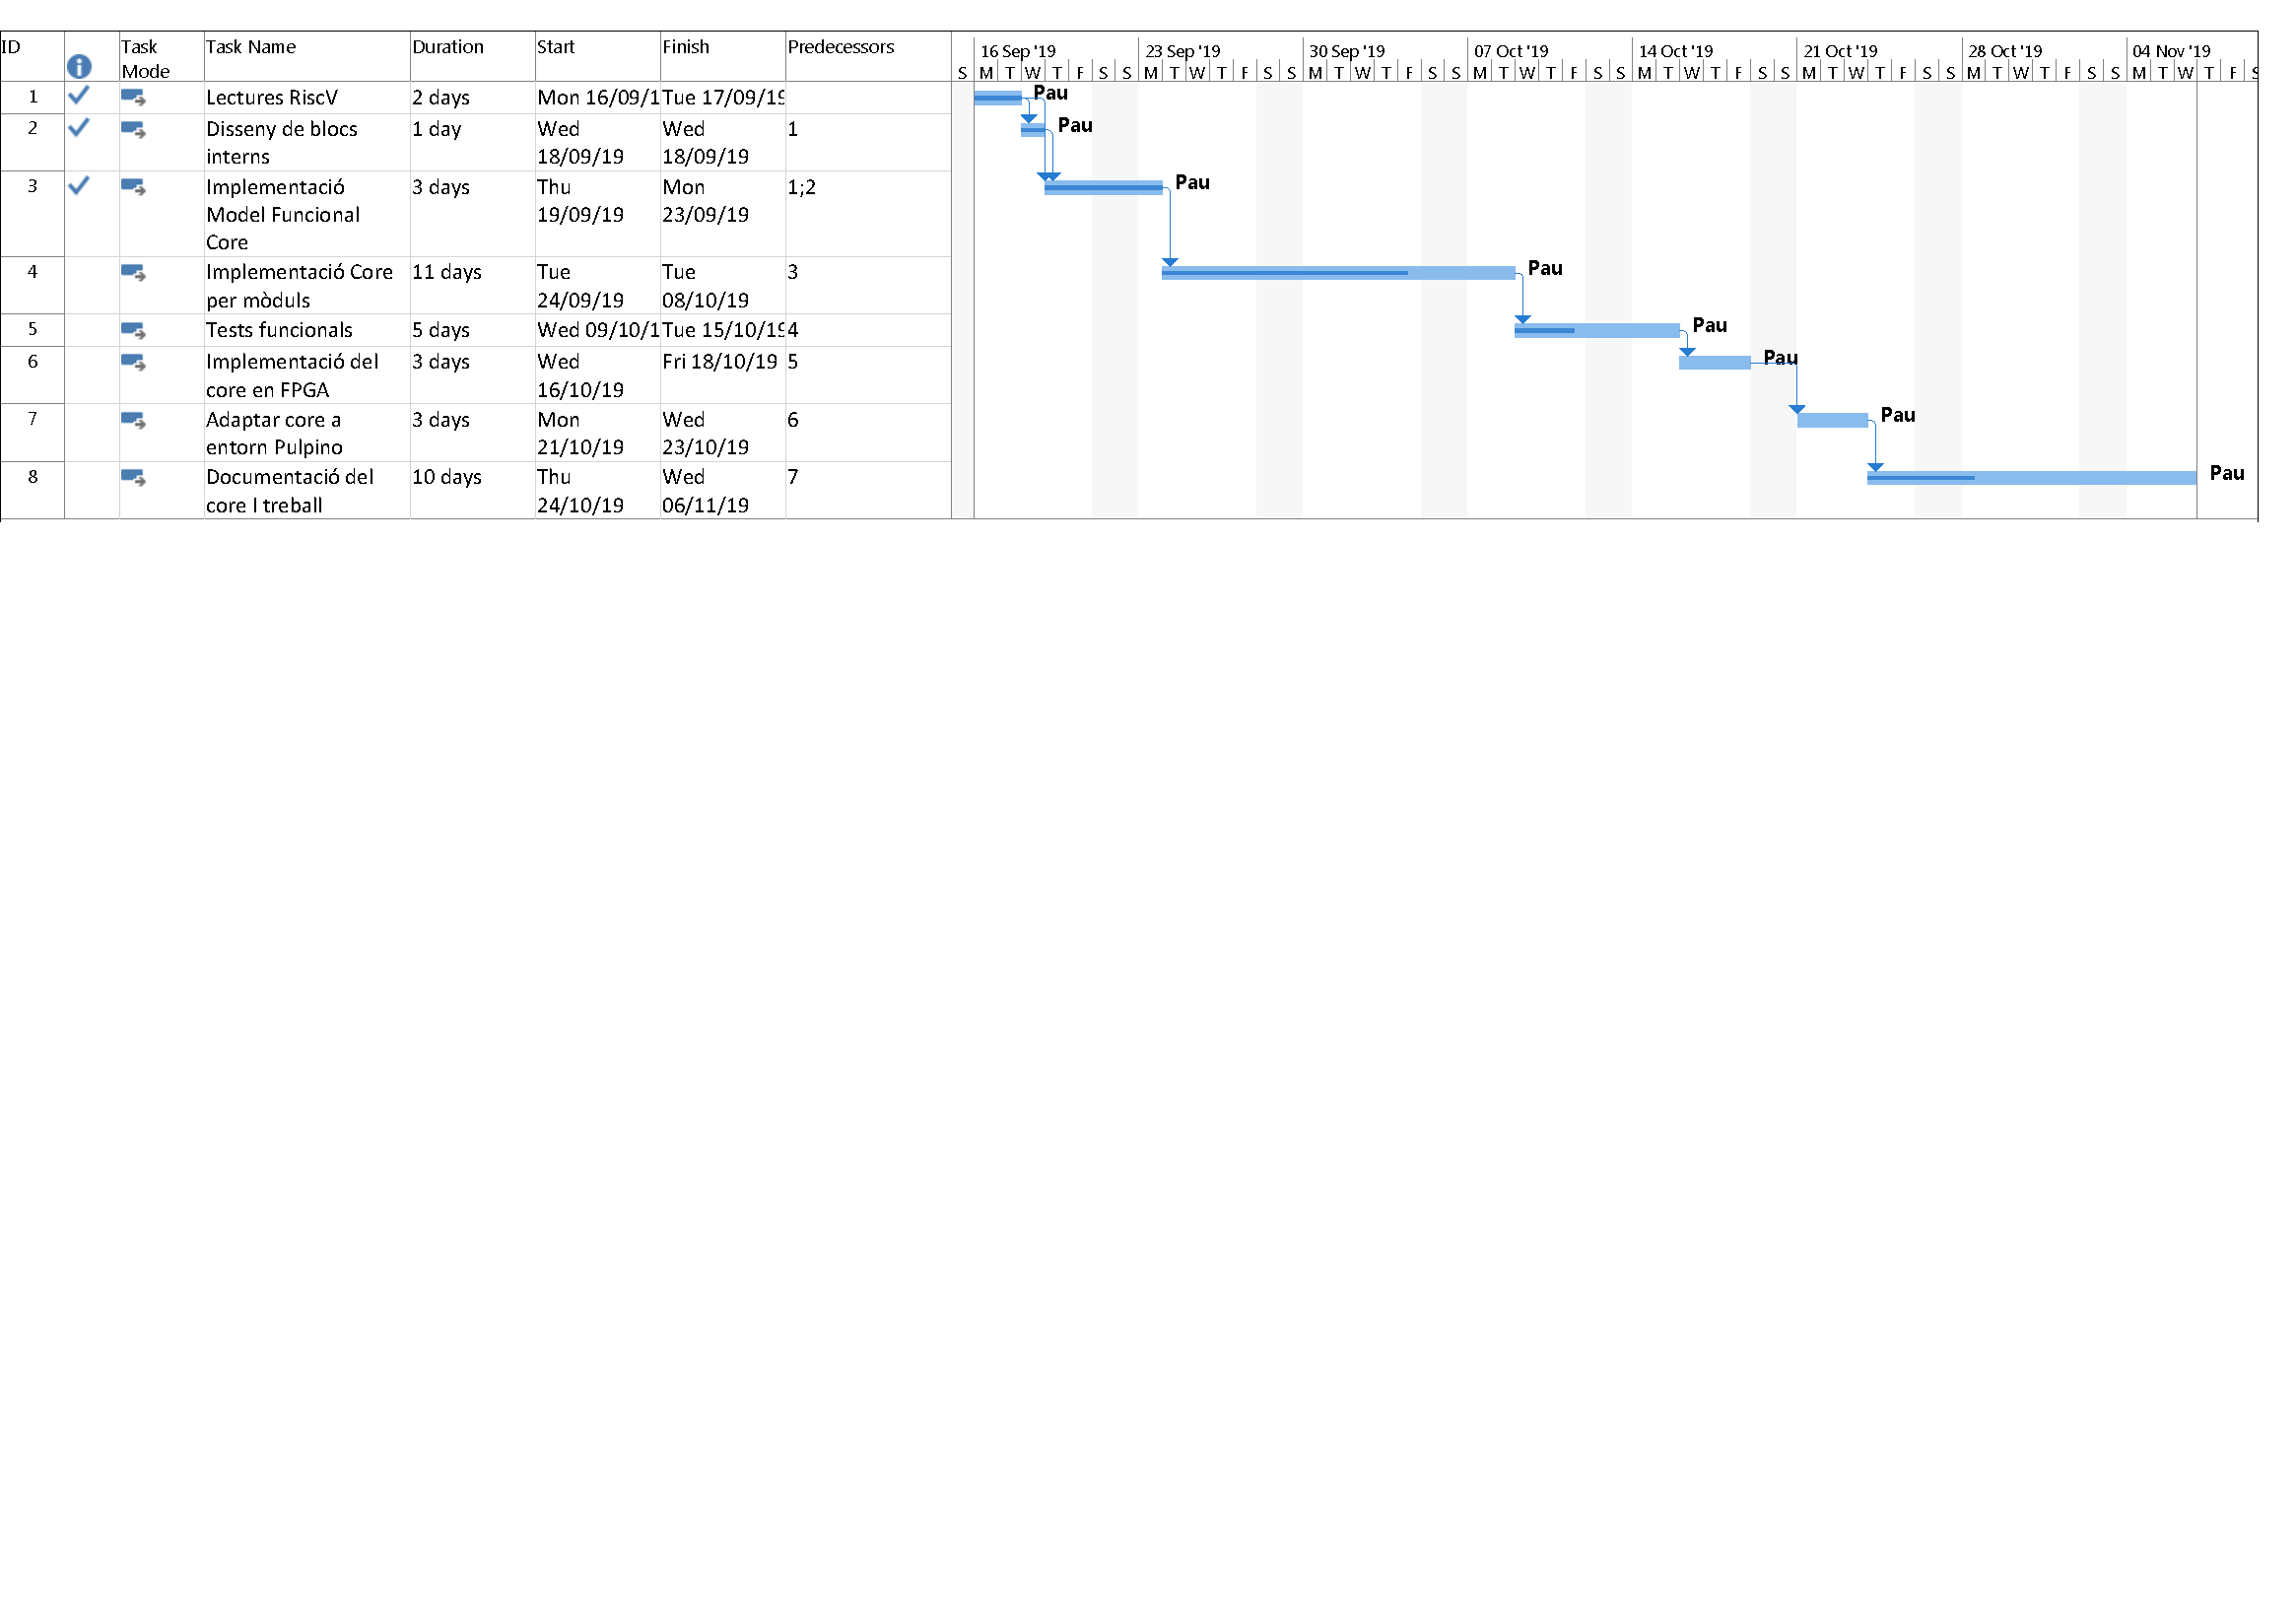
\includegraphics[width=\textwidth]{gantt.pdf}
%\caption{Gantt bàsic amb la planificació a falta de subdividir en tasques.}
%\label{fig:gantt}
%\end{figure}

\section{Canvis}
Després de la reunió del dia 9 de desembre es van proposar les solucions per als problemes abans esmentats. Això permetrà continuar la planificació del informe de seguiment anterior. Analitzant els documents a entregar s'ha determinat que el dossier final inclogui una memòria que reculli el disseny del nucli, aquest amb un format més extens al informe final del treball proposat per la guia docent del TFG. S'efectua una proposta del índex amb les seccions que inclourà la memòria del nucli a les posteriors pàgines.



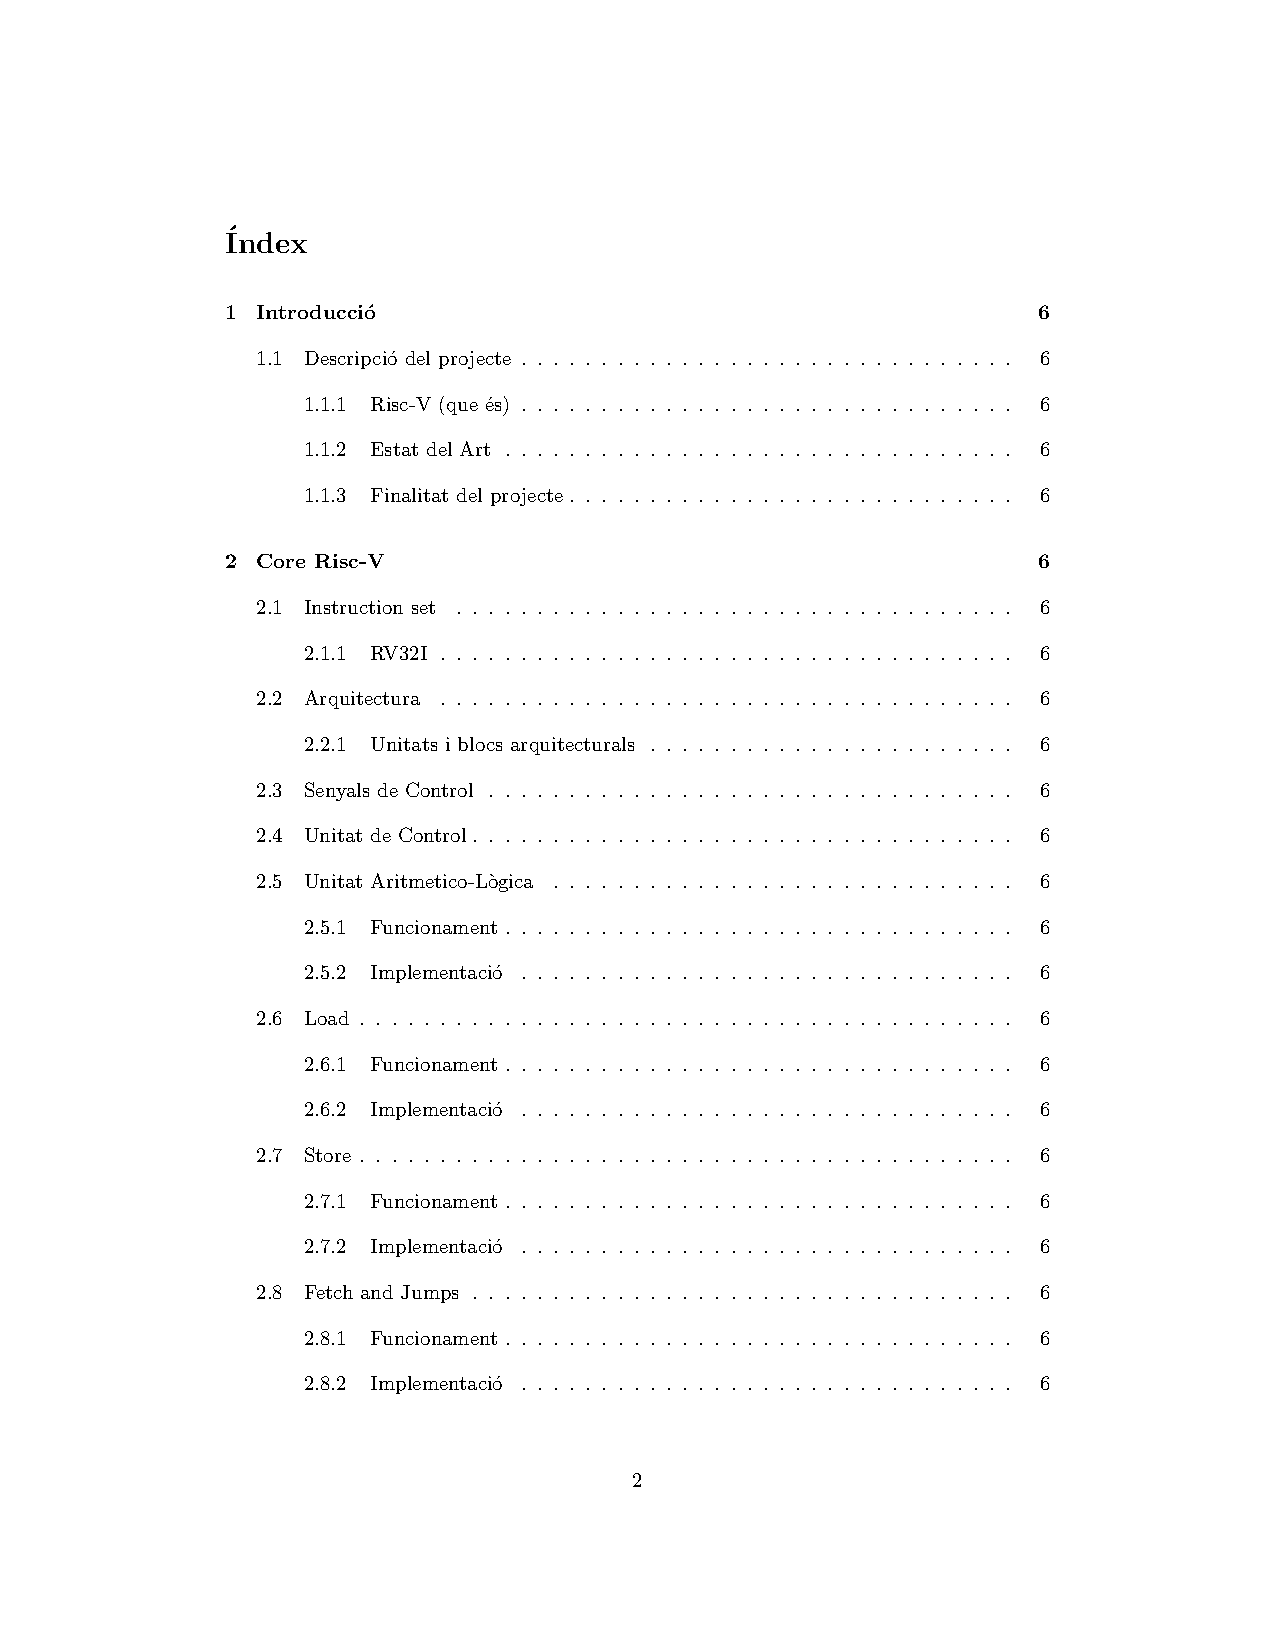
\includepdf[pages={1-},scale=1]{index.pdf}





\bibliographystyle{IEEEtran}
\bibliography{references.bib}


\end{document}
